% !TEX root = isae-beamer-template.tex

% Recall the outline at each section
\begin{frame}
  \frametitle{Serielle Kommunikation über UART}
	    \begin{column}{1\linewidth}
	    	Übersicht über die Hardware-Anbindung UART:\\
	    	Achtung: Robo V1 über \textbf{Segger RTT}
	    	\begin{center}
	    		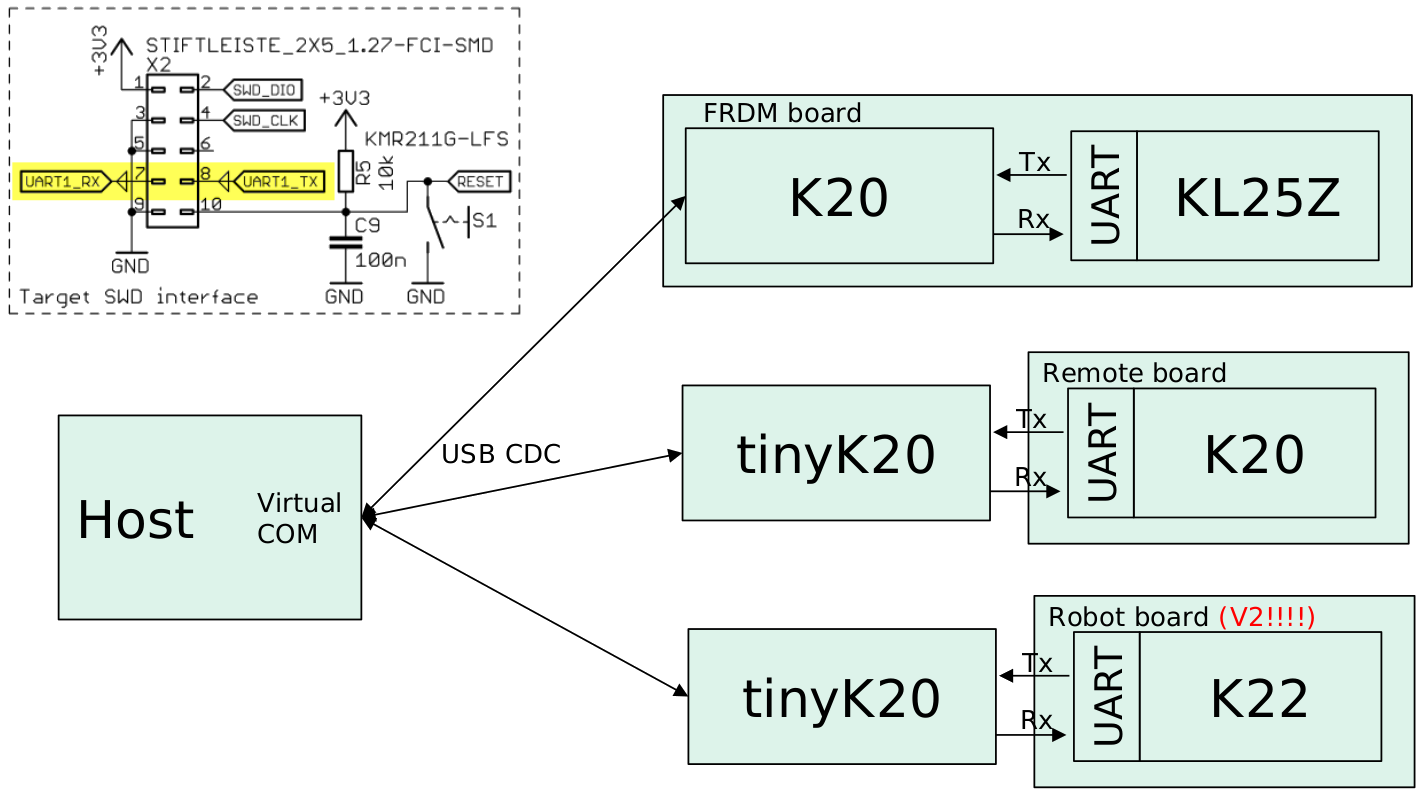
\includegraphics[width=0.8\textwidth]{images/UART_HW_Mapping.png}
	    	\end{center}
	    \end{column}
\end{frame}

\begin{frame}
  \frametitle{Processor Expert Komponenten}
  	\begin{columns}
	    \begin{column}{0.45\linewidth}
	    	\begin{itemize}
	    	\item CLS1:Shell in Processor Expert
	    	\item Blockierendes Senden einschalten
	    	\item WAIT1 verwenden
	    	\item Timeout: Wartezeit zwischen dem Senden. \\0 = blockierend
	    	\item Wait Time: Wenn der Puffer voll ist, wie lange soll gewartet werden?
	    	\item Console Interface: AS1
	    	\end{itemize}
	    \end{column}
	    \begin{column}{0.45\linewidth}
	    	\begin{center}
	    		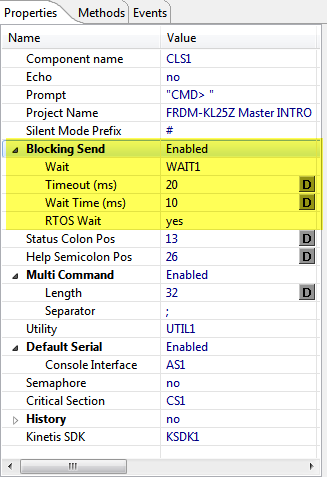
\includegraphics[width=0.8\textwidth]{images/CLS1_shell.png}
	    	\end{center}
	    \end{column}
	\end{columns}
\end{frame}

\begin{frame}
  \frametitle{AS1 Einstellungen}
  	\begin{columns}
	    \begin{column}{0.45\linewidth}
	    	\begin{itemize}
	    	\item Channel: UART0
	    	\item Input buffer size: 32Bit empfohlen
	    	\item Output buffer size: 32Bit empfohlen
	    	\item Receiver: UART0\_RX
	    	\item Transmitter: UART0\_TX
	    	\item Baudrate setzen und mit Terminal abgleichen
	    	\end{itemize}
	    \end{column}
	    \begin{column}{0.45\linewidth}
	    	\begin{center}
	    		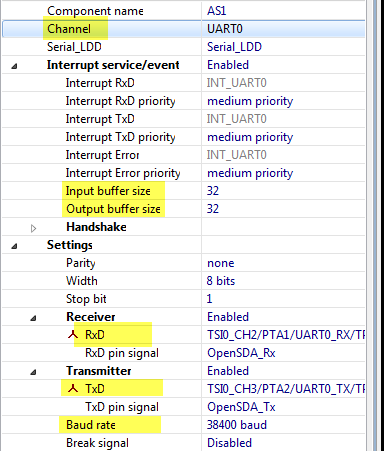
\includegraphics[width=1\textwidth]{images/CLS1_shell_2.png}
	    	\end{center}
	    \end{column}
	\end{columns}
\end{frame}

\begin{frame}[fragile]
  \frametitle{Anschluss am PC/ Notebook}
	    \begin{column}{1\linewidth}
	    	\textbf{Port finden bei Windows:}\\
	    	\begin{center}
	    		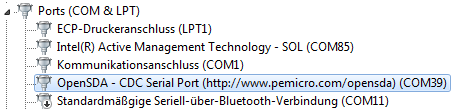
\includegraphics[width=0.8\textwidth]{images/COM_Windows.png}
	    	\end{center}
	    	\textbf{Bei Linux:}\\
	    	Terminal öffnen und den Befehl: 
			\begin{verbatim}
			dmesg | grep tty
			\end{verbatim}
	    	ausführen. (Bei mir \textbf{ttyACM0})
	    	\begin{center}
	    		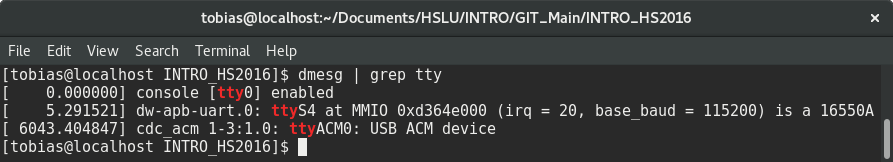
\includegraphics[width=0.8\textwidth]{images/Console_Result_dmesc.png}
	    	\end{center}
	    \end{column}
\end{frame}